\documentclass[11pt]{article}
\usepackage[scaled=0.92]{helvet}
\usepackage{geometry}
\geometry{letterpaper,tmargin=1in,bmargin=1in,lmargin=1in,rmargin=1in}
\usepackage[parfill]{parskip} % Activate to begin paragraphs with an empty line rather than an indent %\usepackage{graphicx}
\usepackage{amsmath,amssymb, mathrsfs,  mathtools, dsfont}
\usepackage{tabularx}
\usepackage{tikz-cd}
\usepackage[font=footnotesize,labelfont=bf]{caption}
\usepackage{graphicx}
\usepackage{xcolor}
%\usepackage[linkbordercolor ={1 1 1} ]{hyperref}
%\usepackage[sf]{titlesec}
\usepackage{natbib}
\usepackage{../../Tianpei_Report}

%\usepackage{appendix}
%\usepackage{algorithm}
%\usepackage{algorithmic}

%\renewcommand{\algorithmicrequire}{\textbf{Input:}}
%\renewcommand{\algorithmicensure}{\textbf{Output:}}



\begin{document}
\title{Lecture 20: Curvature}
\author{ Tianpei Xie}
\date{Oct. 26th., 2022}
\maketitle
\tableofcontents
\newpage
\section{Local Invariants}
\begin{itemize}
\item \begin{remark}
For any geometric structure defined on smooth manifolds, it is of great interest to address \emph{\textbf{the local equivalence question}}: Are all examples of the structure locally equivalent to each other (under an appropriate notion of local equivalence)? 

The most important technique for proving that \emph{two geometric structures} are \emph{\textbf{not locally equivalent}} is to find \emph{\textbf{local invariants}}, which are quantities that must be preserved by local equivalences. In order to address the general problem of local equivalence of Riemannian or pseudo-Riemannian metrics, we will define a local invariant for all such metrics called \emph{\textbf{curvature}}. 

Initially, its definition will have nothing to do with \emph{\textbf{the curvature of curves}}, but later we will see that the two concepts are intimately related.
\end{remark} 


\begin{figure}
\begin{minipage}[htb]{1\linewidth}
  \centering
  \centerline{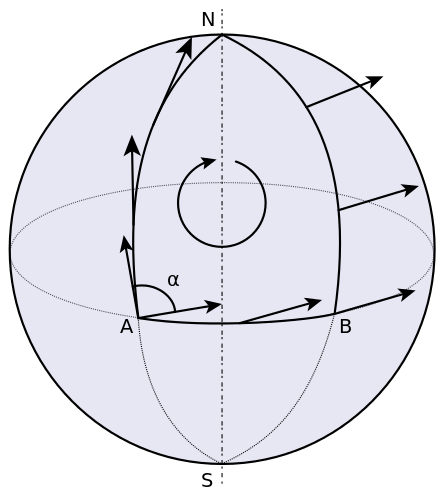
\includegraphics[scale = 0.4]{Parallel_Transport.png}}
\end{minipage}
\caption{\footnotesize{\textbf{Result of parallel transport along the $x^1$-axis and the $x^2$-coordinate lines \citep{lee2018introduction}}}}
\label{fig: parallel_transport_along_two_axis}
\end{figure}

\item \begin{remark}
The \emph{sphere} and the \emph{plane} are \emph{not locally isometric}. The key idea is that \emph{every tangent vector} in the plane can be extended to a \emph{parallel
vector field}, so every Riemannian manifold that is \emph{locally isometric to} $\bR^2$ must have the same property locally.
\end{remark}

\item \begin{remark}
Given a Riemannian $2$-manifold M, here is one way to attempt to construct \emph{\textbf{a parallel extension}} of a vector $z \in T_{p}M$ working in any smooth local coordinates
$(x^1, x^2)$ centered at $p$:
\begin{enumerate}
\item first \emph{\textbf{parallel transport}} $z$ \emph{\textbf{along the $x^1$-axis}};
\item then \emph{\textbf{parallel transport}} the \textit{resulting vectors} along the coordinate lines \emph{\textbf{parallel to the $x^2$-axis}} (Fig. \ref{fig: parallel_transport_along_two_axis}). 
\end{enumerate} By construction,  the resulting \emph{vector field $Z$ is \textbf{\underline{parallel along every $x^2$-coordinate line}} and \textbf{along} the $x^1$-axis}.

The question is \emph{whether this vector field is \underline{\textbf{parallel along $x^1$-coordinate lines}} other than the $x^1$-axis}, or in other words, whether $\conn{\partial_1}{Z} \equiv 0$. Observe that $\conn{\partial_1}{Z}$ \emph{\textbf{vanishes}} when $x^2 = 0$. If we could show that
\begin{align}
\conn{\partial_2}{\conn{\partial_1}{Z}} = 0 \label{eqn: euclidean_2_manifold_parallel_transport_x_1_zero}
\end{align} then it would follow that $\conn{\partial_1}{Z} \equiv 0$, because \emph{\textbf{the zero vector field}} is \emph{the \textbf{unique} parallel transport of \textbf{zero}} along the $x^2$-curves. If we knew that
\begin{align}
\conn{\partial_2}{\conn{\partial_1}{Z}} = \conn{\partial_1}{\conn{\partial_2}{Z}} \label{eqn: euclidean_2_manifold_parallel_transport_x_1_x_2}
\end{align}
then \eqref{eqn: euclidean_2_manifold_parallel_transport_x_1_zero} would follow immediately, because $\conn{\partial_2}{Z} \equiv 0$ everywhere by construction. 
\end{remark}

\item \begin{remark}
Let us look more closely at the quantity $\overline{\nabla}_{X}{\overline{\nabla}_{Y}}Z  - \overline{\nabla}_{Y}{\overline{\nabla}_{X}}Z$ when $X$, $Y$, and $Z$ are smooth vector fields.
\begin{align*}
\overline{\nabla}_{X}{\overline{\nabla}_{Y}}Z &= \overline{\nabla}_{X}{(Y(Z^k)\partial_k)} = X\paren{Y^{j} \partial_j(Z^k)}\partial_k= XY(Z^k)\partial_k\\
\overline{\nabla}_{Y}{\overline{\nabla}_{X}}Z &= YX(Z^k)\partial_k\\
\overline{\nabla}_{X}{\overline{\nabla}_{Y}}Z  - \overline{\nabla}_{Y}{\overline{\nabla}_{X}}Z &= (XY - YX)(Z^k)\partial_k = [X, Y](Z^k)\partial_k = \overline{\nabla}_{[X, Y]}{Z}\\
\Rightarrow \overline{\nabla}_{X}{\overline{\nabla}_{Y}}Z  - \overline{\nabla}_{Y}{\overline{\nabla}_{X}}Z &=\overline{\nabla}_{[X, Y]}{Z}.
\end{align*} Recall that a Riemannian manifold is said to be \emph{\textbf{flat}} if it is \emph{\textbf{locally isometric}} to a \emph{\textbf{Euclidean space}}, that is, if every point has a neighborhood that is \emph{\textbf{isometric}} to an open set in $\bR^n$ with its \emph{\textbf{Euclidean metric}}. 

We say that a \emph{\textbf{connection}} $\nabla$ on a smooth manifold $M$ satisfies \underline{\emph{\textbf{the flatness criterion}}} if whenever $X, Y, Z$ are smooth vector fields defined on an open subset of $M$, the following identity holds:
\begin{align}
\conn{X}{\conn{Y}{Z}} - \conn{Y}{\conn{X}{Z}}  = \conn{[X, Y]}{Z} \label{eqn: flatness_criterion}
\end{align}
\end{remark}

\item \begin{remark}
The geometric interpretation of the term $\conn{X}{\conn{Y}{Z}}$ is the \emph{two-step process}:
\begin{enumerate}
\item First, \emph{\textbf{parallel transport}} of $Z$ along \emph{the \textbf{flow} of vector field} $Y$;
\item Then, \emph{\textbf{parallel transport}} of $Z$ along \emph{the \textbf{flow} of vector field} $X$
\end{enumerate} Then the resulting vector field is $\conn{X}{\conn{Y}{Z}}$.
\end{remark}

\item \begin{proposition}
If $(M,g)$ is a \textbf{flat} Riemannian or pseudo-Riemannian manifold, then its \textbf{Levi-Civita connection} satisfies \textbf{the flatness criterion}.
\end{proposition}
\end{itemize}

\section{The Curvature Tensor}
\subsection{Definitions}
\begin{itemize}
\item \begin{definition}
Let $(M,g)$ be a Riemannian or pseudo-Riemannian manifold, and define a map $R: \frX(M) \times \frX(M) \times \frX(M) \rightarrow \frX(M)$ by
\begin{align}
R(X, Y)Z &= \conn{X}{\conn{Y}{Z}} - \conn{Y}{\conn{X}{Z}}  -  \conn{[X, Y]}{Z} \label{eqn: curvature_def}
\end{align}
\end{definition}

\item The following proposition make sure this multilinear map defines a $(1,3)$-tensor field
\begin{proposition}
The map $R$ defined above is \textbf{multilinear} over $\cC^{\infty}(M)$, and thus defines a \textbf{$(1,3)$-tensor field} on $M$.
\end{proposition}

\item \begin{definition}
For each pair of vector fields $X, Y \in \frX(M)$, the map $R(X,Y): \frX(M) \rightarrow \frX(M)$ given by $Z \mapsto R(X,Y)Z$ is a \emph{\textbf{smooth bundle endomorphism}} of $TM$, called \emph{\textbf{the curvature endomorphism determined by $X$ and $Y$}}.

The \emph{\textbf{tensor field $R$}} itself is called \emph{\textbf{the (Riemann) curvature endomorphism}} or the \underline{\emph{\textbf{$(1, 3)$-curvature tensor}}}. 
\end{definition}

\item \begin{remark} (\emph{\textbf{Coordinate Representation of the $(1,3)$-Curvature Tensor}})\\
We adopt the convention that \emph{\textbf{the last index is the contravariant (upper) one}}. This is contrary to our default assumption that \emph{covector arguments come first}. Thus, for example, \emph{the curvature endomorphism} can be written in terms of local coordinates $(x^i)$ as
\begin{align*}
R &= R_{i,j,k}^{l}\,dx^i \otimes dx^j \otimes dx^k \otimes \partdiff{}{x^l},
\end{align*} where the coefficients $R_{i,j,k}^{l}$ are defined by
\begin{align*}
R\paren{\partdiff{}{x^i}, \partdiff{}{x^j}}\partdiff{}{x^k} &= R_{i,j,k}^{l}\, \partdiff{}{x^l}.
\end{align*}
\end{remark}

\item \begin{remark} (\emph{\textbf{Understanding the Geometric Meaning of the $(1,3)$-Curvature Tensor}})\\
The  $(1,3)$-tensor $R(X, Y)Z$ describes \emph{the \textbf{difference} of  resulting \textbf{vector fields}} after \emph{\textbf{parallel transporting}} vector field $Z$ through \emph{\textbf{two different routes}}: 
\begin{enumerate}
\item First \emph{\textbf{parallel transporting}} along \emph{\textbf{the flow of $Y$}}, then \emph{\textbf{parallel transporting}} along \emph{\textbf{the flow of $X$}}, the resulting vector field is $ \conn{X}{\conn{Y}{Z}}$;
\item First \emph{\textbf{parallel transporting}} along \emph{\textbf{the flow of $X$}}, then \emph{\textbf{parallel transporting}} along \emph{\textbf{the flow of $Y$}}, the resulting vector field is $ \conn{Y}{\conn{X}{Z}}$;
\end{enumerate}
The last term $\conn{[X, Y]}{Z}$ provides additional \emph{\textbf{correction}} if $X$ and $Y$ are \emph{\textbf{not orthorgonal}}.

Thus $R(X, Y)Z = \conn{X}{\conn{Y}{Z}} - \conn{Y}{\conn{X}{Z}}  -  \conn{[X, Y]}{Z}$ is \emph{\textbf{close related to}} \emph{the \textbf{angle} of these \textbf{two resulting vector fields}}. If the surface is \emph{\textbf{flat}}, this angle should be \emph{\textbf{zero}} since \emph{the vector field \textbf{does not rotate}} during the transport and it is \emph{\textbf{regardless of the path it takes}}. On the other hand, if \emph{\textbf{the surface bends}}, then the vector field \emph{will rotate} during the parallel transport and thus traversing through different paths will cause the vector field \emph{points to different directions} in final destination, i.e. the angle is not zero.
\end{remark}

\item \begin{proposition} (\textbf{The Riemann Curvature via Coefficients of Connection}) \citep{lee2018introduction}\\
Let $(M,g)$ be a Riemannian or pseudo-Riemannian manifold. In terms of any smooth local coordinates, the components of the $(1,3)$-curvature tensor are given by
\begin{align}
R_{i,j,k}^l &= \partial_i \Gamma_{j,k}^{l} -\partial_j \Gamma_{i,k}^{l} + \Gamma_{j,k}^{m}\Gamma_{i,m}^{l}- \Gamma_{i,k}^{m}\Gamma_{j,m}^{l}. \label{eqn: rieman_curvature_13_tensor_coefficient}
\end{align}
\end{proposition}

\item \begin{remark}
The curvature endomorphism also measures \emph{\underline{\textbf{the failure}} of \textbf{second covariant derivatives} along \textbf{families} of curves to \underline{\textbf{commute}}}. Given a smooth one-parameter \emph{family of curves} $\Gamma: J \times I \rightarrow M$, recall that the velocity fields $\partial_{t}\Gamma(s,t) = (\Gamma_s)'(t)$ and $\partial_{s}\Gamma(s,t) = (\Gamma^{(t)})'(s)$ are smooth vector fields along $\Gamma$.

\begin{proposition}
Suppose $(M,g)$  is a smooth Riemannian or pseudo-Riemannian manifold and  $\Gamma: J \times I \rightarrow M$  is a smooth one-parameter \textbf{family} of curves in $M$.
Then for every smooth vector field $V$ along $\Gamma$,
\begin{align}
D_{s}D_{t}V - D_{t}D_{s}V &= R(\partial_s\,\Gamma, \partial_t\,\Gamma)V  \label{eqn: rieman_curvature_2nd_covariant_deriv_not_commute}
\end{align}
\end{proposition}
\end{remark}

\item \begin{definition}
We define the \underline{\emph{\textbf{(Riemann) curvature tensor}}} to be the \underline{\emph{$(0,4)$-tensor field}} $Rm = R^{\flat}$ (also denoted by
$Riem$ by some authors) obtained from the $(1,3)$-curvature tensor $R$ by \emph{\textbf{lowering its last index}}. Its \emph{action} on vector fields is given by
\begin{align}
Rm(X, Y, Z, W) &:= \inn{R(X, Y)Z}{W}_{g} \label{eqn: rieman_curvature_tensor_on_vector_field}
\end{align} This quanitity measures the angle between $R(X, Y)Z$ and $W$.
\end{definition}

\item \begin{remark} (\emph{\textbf{Coordinate Representation of the Riemann Curvature Tensor}})\\
In terms of any smooth local coordinates, it is written
\begin{align*}
Rm &= R_{i,j,k,l}\,dx^i \otimes dx^j \otimes dx^k \otimes dx^l,
\end{align*}
where $ R_{i,j,k,l} = g_{l,m}R_{i,j,k}^{m}$.  We also see that 
\begin{align}
R_{i,j,k,l} &= g_{l,m}\paren{\partial_i \Gamma_{j,k}^{m} -\partial_j \Gamma_{i,k}^{m} + \Gamma_{j,k}^{p}\Gamma_{i,p}^{m}- \Gamma_{i,k}^{p}\Gamma_{j,p}^{m}}. \label{eqn: rieman_curvature_tensor_coefficient}
\end{align}
\end{remark}

\item \begin{proposition}
The \textbf{curvature tensor} is a \underline{\textbf{local isometry invariant}}: if $(M,g)$ and $(\widetilde{M}, \widetilde{g})$ are Riemannian or pseudo-Riemannian manifolds and $\varphi: M \rightarrow \widetilde{M}$ is a local isometry, then $\varphi^{*}\widetilde{Rm} = Rm$.
\end{proposition}
\end{itemize}
\subsection{Flat Manifolds}
\subsection{Symmetries of the Curvature Tensor}

\section{Ricci and Scalar Curvatures}
\subsection{The Ricci Identities}
\subsection{Ricci and Scalar Curvatures}

\section{The Weyl Tensor}
\section{Curvatures of Conformally Related Metrics}

\newpage
\bibliographystyle{plainnat}
\bibliography{book_reference.bib}
\end{document}